\chapter{Marco teórico: Teoría de sistemas, caos y simulación}

La teoría general de sistemas es un enfoque interdisciplinario que se utiliza para comprender la complejidad bajo diferentes contextos y tiene dos pilares fundamentales: todo puede ser concebido como un sistema y las conexiones entre las partes son esenciales para su funcionamiento.

Independientemente de la naturaleza o su escala, cualquier entidad o fenómeno puede entenderse como un conjunto de elementos interconectados que trabajan en conjunto para lograr un objetivo. Por otro lado, las diferentes interacciones que se dan entre estos elementos, ya sea de materia, energía o información, son las que permiten que funcione un sistema \cite{dinamicos}.

Como no es práctico hacer experimentos en la naturaleza, que se define como todo proceso que se puede observar \cite{naturaleza}, necesitamos modelos que nos ayuden a probar cómo responde un proceso a ciertos estímulos que son importantes para el observador. En este capítulo se introducen elementos de la teoría general de sistemas y cuáles son los métodos y técnicas para la simulación de sistemas complejos.

\section{Sistemas}

Antes de adentrarnos en la definición de sistemas complejos y simulación, es necesario conocer qué es proceso, modelo y sistema.

\begin{definition}
	
	Un proceso es cualquier cosa que se encuentre en la naturaleza y que tiene un propósito que depende del observador.
	
\end{definition}

Un proceso es un ente real que mapea diferentes estímulos o entradas en salidas o respuestas a esos estímulos.

\begin{definition}
	
	Un modelo es cualquier abstracción de un proceso que realiza un observador.
	
\end{definition}

Los modelos son inherentes al proceso original que los generó, es decir, se puede utilizar el mismo modelo para múltiples procesos que comparten ciertas propiedades. Por ejemplo, un modelo que examina las fuerzas que interactúan en un objeto que se encuentra en caída libre no depende de especificaciones del objeto como su color o su forma.

Los modelos permiten probar las respuestas de un proceso a estímulos de interés para el observador. Siguiendo el ejemplo de caída libre, no es necesario soltar múltiples objetos de diferentes alturas para identificar las fuerzas que están interactuando; únicamente es necesario probar las diferentes entradas dentro del mismo modelo. Además, la calidad de un modelo se determina si las salidas producidas son similares a las que produciría el proceso.

Finalmente, un sistema es un conjunto de partes interrelacionadas que actúan de manera coordinada y cumplen una función en específico. O dicho de otro modo: 

\begin{definition}
	
	Un sistema es un modelo matemático que cumple con ciertos axiomas que lo caracterizan.
	
\end{definition}

De acuerdo con \cite{sistema_1}, los sistemas se caracterizan principalmente por

\begin{itemize}
	
	\item Estar compuestos por elementos internos independientes que pueden organizarse en subsistemas.
	
	\item Operar de manera organizada para cumplir un objetivo.
	
	\item Tener elementos que se puedan distinguir como parte del sistema o del ambiente.
	
	\item Existir en un marco temporal.
	
\end{itemize}

\subsection{Clasificación de sistemas}

Los sistemas se pueden clasificar según su relación con el entorno, su origen, composición, comportamiento, etc. Estas son las clasificaciones que puede tener: 

\subsubsection{Sistemas naturales y artificiales}

Un sistema es natural si no requiere de intervención humana para ser creado; son regidos por leyes físicas, químicas, biológicas y psicológicas. El sistema solar, el sistema respiratorio o el sistema cardiaco son algunos ejemplos. 

Por otro lado, los sistemas artificiales son aquellos creados por los humanos y que cumplen un propósito. Estos tienen un dominio en el conocimiento, la ingeniería y las interacciones sociales. Por ejemplo, las calculadoras, el sistema educativo o las relaciones comerciales \cite{natural_artificial}.

\subsubsection{Sistemas continuos y discretos en el tiempo}

Se dice que un sistema es continuo en el tiempo si sus entradas y salidas son señales continuas en esa variable.

Por otro lado, es discreto si transforma señales discretas en el tiempo en señales de salida discretas en el tiempo \cite{continuo_discreto}.

\subsubsection{Sistemas estáticos y dinámicos}

Un sistema estático o sin memoria es aquel que permanece en un estado constante o inmutable, es decir, no cambia con el tiempo. Se dice entonces que un sistema es estático si su salida en cualquier instante de tiempo depende solamente de entradas en ese mismo momento y, de acuerdo con \cite{estatico_dinamico}, estos se caracterizan por:

\begin{itemize}
	
	\item Inmutabilidad: No cambia con el tiempo y mantiene su estado constante.
	
	\item Estabilidad: Es sencillo de predecir y controlar su comportamiento.
	
	\item Simplicidad: Usualmente son más sencillos en diseño y operación, lo que facilita su implementación. 
	
\end{itemize} 

Por otro lado, un sistema dinámico o con memoria es aquel que cambia con el tiempo. Estos tienen la capacidad de adaptarse y responder ante diferentes condiciones de entrada. En otras palabras, es aquel cuya salida en un instante de tiempo depende de entradas en otros instantes y posiblemente de entradas en ese mismo instante. Este se caracteriza por:

\begin{itemize}
	
	\item Cambio en el tiempo: Se adapta ante diferentes situaciones y entradas.
	
	\item Flexibilidad: Responde ante diferentes condiciones y requisitos.
	
	\item Complejidad: Son más complejos en diseño y operación debido a su capacidad de cambio.
	
\end{itemize}

Aunque en la naturaleza no podemos encontrar procesos estáticos, en ocasiones resulta impráctico modelarlos como sistemas dinámicos \cite{dinamicos}.

Este es un ejemplo de un sistema estático:

\begin{equation*}
	y[n] = 2x[n] + 2
\end{equation*}

Ya que en cualquier instante de tiempo particular $n_0$, el valor de $y[n]$ depende solamente del valor de $x[n]$ en ese mismo instante de tiempo $n_0$.

Por otro lado, este es un ejemplo de un sistema dinámico:

\begin{equation*}
	y[n] = x[n] + x[n-1]
\end{equation*}

Ya que el valor de $y[n]$ en el tiempo $n_x$ depende del de $x[n]$ en $n_1$ y en $n_{n-1}$.

\subsubsection{Sistemas deterministas y estocásticos}

Un sistema determinista es un sistema en donde las mismas entradas producirán invariablemente las mismas salidas. No se contempla la existencia del azar, variables aleatorias ni principio de incertidumbre.

Por otro lado, un sistema estocástico es aquel que se rige por el azar. El resultado depende de probabilidades que cambian o pueden variar en función del tiempo \cite{probabilistico}.

No hay que confundir los sistemas estocásticos con los sistemas caóticos. En los sistemas estocásticos existe una variable aleatoria que impide que las mismas entradas tengan las mismas salidas. Los sistemas caóticos son deterministas, pero determinar el sistema en evoluciones futuras resulta complicado. 

\subsubsection{Sistemas abiertos y cerrados}

Un sistema es abierto si puede intercambiar materia, energía o información con su entorno. Tienen una interacción activa con el mundo que los rodea o con su ambiente. Estas influencias externas pueden ajustar las respuestas del propio sistema y se caracterizan por:

\begin{itemize}
	
	\item Adaptabilidad: Pueden ajustar el comportamiento y estructuras internas para mantener su funcionamiento y equilibrio en respuesta a perturbaciones externas.
	
	\item Homeostasis dinámica: Pueden mantener un equilibrio interno a lo largo del tiempo.
	
	
	
	\item Entradas y salidas: Sus entradas adquieren información del entorno y las salidas le devuelven una respuesta.
	
\end{itemize}

Por su parte, los sistemas cerrados se encuentran aislados de su entorno. Tiene límites que actúan como barreras para el intercambio de materia, energía o información. Estos operan de forma autocontenida y no tienen una interacción con el entorno que los rodea.

Siguiendo a \cite{tgs}, todas las fluctuaciones y cambios dependen únicamente de los elementos que se encuentren dentro del sistema. Estos sistemas tienden a mantener su estructura y equilibrio interno de manera constante; esto se debe principalmente a que:

\begin{itemize}
	
	\item La frontera impide interacción significativa con el entorno, por lo que no se ve afectado el funcionamiento interno.
	
	\item Conservan la energía y la materia que los contienen, lo que contribuye a la estabilidad de la estructura y el equilibrio.
	
\end{itemize}

\section{Propiedades fundamentales de los sistemas}

Las propiedades de los sistemas dependen de su dominio. El dominio de un sistema es el campo sobre el cual se extiende su influencia \cite{dominio}. A continuación se listan las propiedades fundamentales de los sistemas.

\subsection{Causalidad}

Un sistema es causal si su señal de salida en cualquier momento depende solamente de las entradas en ese instante específico o en instantes anteriores. Por ejemplo, el siguiente es un sistema que depende de entradas futuras:

\begin{equation*}
	y(t) = x(t + 1)
\end{equation*}

Los sistemas anticausales tienen aplicaciones en imágenes, reconocimiento de voz, datos geológicos, etc. En la naturaleza, todos los procesos son causales \cite{dinamicos}.

\subsection{Invertibilidad}

Un sistema es invertible si a distintas entradas le corresponden distintas salidas, es decir, si podemos definir las entradas conociendo la salida del sistema. 

Si el sistema es invertible, podemos definir un sistema inverso que reciba como entrada la salida del sistema original y devuelva la entrada. Por lo que, si conectamos el sistema inverso a la salida del sistema original, obtendremos como resultado la entrada \cite{dinamicos}.

\subsection{Estabilidad}

Se denomina punto de equilibrio a un sistema dinámico a aquel en que la variable de interés permanece constante con todas sus derivadas iguales a cero.

Supóngase que se tiene un sistema dinámico autónomo, es decir, sin señales de entrada, y que este se encuentra en un punto de equilibrio. Se define como un punto de equilibrio estable si, al dejar evolucionar libremente el sistema a partir de una condición inicial en una vecindad del punto de equilibrio, el sistema regresa a dicho punto. Sí, por el contrario, el sistema se aleja, entonces es un punto de equilibrio inestable \cite{dinamicos}.

En la figura \ref{fig:estabilidad} se ilustran ambos puntos de equilibrio. Si una pelota se coloca en una vecindad del punto de equilibrio, en el caso \ref{fig:estabilidad1}, la pelota regresará eventualmente al punto de equilibrio, mientras que en el caso \ref{fig:estabilidad2} la pelota se alejará.

\begin{figure}[htbp]
	\centering
	\begin{subfigure}[b]{0.30\textwidth}
		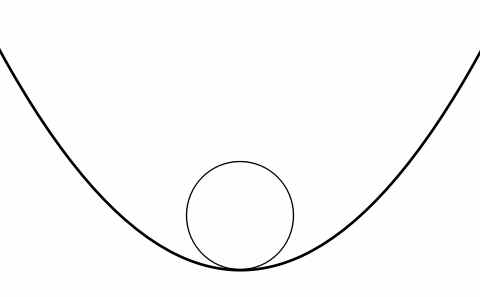
\includegraphics[width=\textwidth]{img/estabilidad1.png}
		\caption{Punto de equilibrio estable.}
		\label{fig:estabilidad1}
	\end{subfigure}
	\begin{subfigure}[b]{0.30\textwidth}
		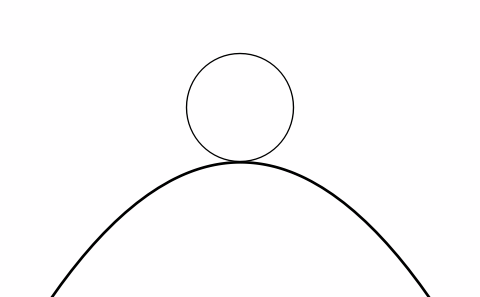
\includegraphics[width=\textwidth]{img/estabilidad2.png}
		\caption{Punto de equilibrio inestable}
		\label{fig:estabilidad2}
	\end{subfigure}
	\caption{Puntos de equilibrio.}
	\label{fig:estabilidad}
	
\end{figure}

Se dice que un sistema es BIBO (\textit{Bounded input bounded output}) estable si a entradas acotadas corresponden salidas acotadas.

Retomando el ejemplo de la figura \ref{fig:estabilidad}, si se aplica un desplazamiento hacia la derecha, en el caso \ref{fig:estabilidad1}, corresponde a una pequeña entrada a la que se le asigna una pequeña salida; por otro lado, si se le aplica una pequeña entrada al caso \ref{fig:estabilidad2}, la diferencia de la respuesta del sistema es mucho más grande \cite{dinamicos}.

\subsection{Invariante en el tiempo}

Se dice que un sistema es invariante en el tiempo si un corrimiento en el tiempo en la señal de entrada causa el mismo corrimiento en el tiempo de la señal de salida del sistema. Si $y(t)$ es la salida de un sistema cuando la entrada es $x(n)$, entonces $y(t - t_0)$ es la salida cuando se aplica la señal de entrada $x(t - t_0)$ \cite{dinamicos}.

\section{Sistemas dinámicos}

Como ya se mencionó, un sistema dinámico es aquel en el cual existe un almacenamiento de energía, materia e información, es decir, es un sistema que posee memoria.

La evolución de un sistema se lleva a cabo con base en estados: el sistema comienza en un estado $x_0$ y la evolución al estado siguiente depende del estado anterior; además, existe una ley que rige su evolución, y, conociendo esta ley, es posible determinar cualquier estado posterior \cite{sis_din}.

De acuerdo con \cite{modelado_sis_det}, podemos definir a un sistema dinámico determinista de la siguiente manera.

\begin{definition}
	
	Un sistema dinámico determinista se define como una colección $D = <T, U, \Omega, Y, Q, \Delta, \varLambda>$ donde: 
	
	\begin{itemize}
		
		\item $T$ es la base del tiempo (el conjunto de valores posibles para la variable $t$).
		
		\item $U$ es el conjunto de valores posibles de la entrada.
		
		\item $\Omega$ es el conjunto de segmentos admisibles de entrada (sus elementos son funciones $\omega : [t_1, t_2] \subset T \to U$).
		
		\item $Y$ es el conjunto de valores de salida.
		
		\item $Q$ es el conjunto de valores posibles de los estados.
		
		\item $\Delta: Q \times \Omega \to Q$ es la función de transición de estados.
		
		\item $\varLambda: Q \to Y$ es la función de salida.
		
	\end{itemize}
	
\end{definition}

La función de transición $\Delta$ se caracteriza por:

\begin{itemize}
	
	\item Dado un segmento de entrada admisible $\omega: [t_1, t_2] \subset T \to U$ y sabiendo que el estado en $t_1$ es $q(t_1) \in Q$, entonces $q(t_2) = \Delta(q(t_1),\omega)$. Es decir, $\Delta$ transforma el estado inicial y la entrada en el estado final. 
	
	\item Dados dos segmentos de entrada admisibles consecutivos $\omega_1: [t_1, t_2] \to U$ y $\omega_2:[t_3, t_4] \to U$, y asumiendo que la concatenación $\omega_1 \circ \omega_2 \in \Omega$, debe cumplirse que $\Delta(q, \omega_1 \circ \omega_2) = \Delta(\Delta(q, \omega_1), \omega_2)$. Esta propiedad garantiza que la evolución del sistema sea compatible con el procesamiento secuencial de entradas.
	
\end{itemize}

\section{Teoría del caos}

De acuerdo con \cite{caos}, el caos trata con sistemas cuyo comportamiento es impredecible a largo plazo. Suele ser asociado a sistemas impredecibles o que no tienen un orden, pero en teoría del caos se refiere a todos aquellos sistemas deterministas cuya predicción en instantes de tiempo futuro se vuelve impredecible. 

Las condiciones iniciales suelen contener errores que incrementarán exponencialmente con el tiempo, lo que se conoce como sensibilidad a las condiciones iniciales, haciendo imposible la predicción a largo plazo. Estos se conocen como sistemas caóticos.

\begin{definition}
	
	Sea $X$ un espacio métrico y sea $\phi: X \to X$ una aplicación continua. Se dice que un sistema es caótico si cumple las siguientes condiciones:
	
	\begin{itemize}
		
		\item La aplicación $\phi: X \to X$ es topológicamente transitiva. 
		
		\item El conjunto de puntos de $\phi$ es denso en el atractor. 
		
		\item La aplicación $\phi: X \to X$ tiene dependencias sensitivas a las condiciones iniciales. 
		
	\end{itemize}	
	
\end{definition}

El hecho de que la aplicación sea topológicamente transitiva implica que el atractor caótico es irreducible, es decir, si iteramos la función $\phi$ un número determinado de veces (evolucionar el sistema durante un periodo de tiempo suficiente), se puede acceder a cualquier punto del atractor desde cualquier otro.

Si el conjunto de puntos es denso en el atractor, entonces cualquier punto en el espacio está arbitrariamente cerca de una órbita periódica. 

Finalmente, la sensibilidad a las condiciones iniciales refleja el hecho de que en un sistema caótico, dos trayectorias que inician relativamente cerca acabarán comportándose de una forma muy diferente a largo plazo. 

\subsection{Exponentes de Lyapunov}

Los exponentes de Lyapunov miden la sensibilidad de las condiciones iniciales y cuantifican la estabilidad o inestabilidad de las trayectorias en el espacio de fases al sufrir una perturbación ligera. Supongamos que tenemos dos trayectorias muy próximas separadas por una distancia $\delta \epsilon_0$; entonces la distancia entre ellas diverge de la forma:

\begin{equation}
	\delta_\epsilon(t) \sim \delta \epsilon_0 e^{\lambda t}
\end{equation}

Donde $\lambda$ es el exponente de Lyapunov. Es decir, mide la tasa de separación entre dos trayectorias muy cercanas en el espacio de fases. En un espacio de fases $n$-dimensional, existen $n$ exponentes de Lyapunov, lo que se conoce como espectro de Lyapunov. 

\subsection{Atractores}

En un espacio disipado, la región del espacio de fases que atrae a las trayectorias vecinas se conoce como atractor. Es un subconjunto en el espacio de fases, es decir, un conjunto de estados a los que tiende a evolucionar el sistema en función de las condiciones iniciales.

\begin{definition}
	
	Sea $X$ el espacio de fases de un sistema dinámico disipado y sea $\phi_t: X \to X$ la transformación que describe el movimiento. Se dice que $A \subset X$ es un atractor si verifica las siguientes condiciones:
	
	\begin{itemize}
		
		\item $\exists U$ entorno de $A$, llamado cuenca de atracción de $A$, tal que $\forall V$ abierto con $A \subset V$, existe un $T_0$ tal que $\phi_t(U) \subset V, \forall t > T_0$.
		
		\item $\phi_t(A) = A, \forall t > 0$
		
		\item $\nexists S \subset A$ subconjunto propio no vacío que satisfaga las dos propiedades anteriores.
		
	\end{itemize} 
	
\end{definition} 

Es decir, un punto que se encuentra en el atractor no puede salir de ahí y, además, existe una órbita alrededor del atractor en donde, para cualquier tiempo, la trayectoria permanece en la órbita.

\subsubsection{Tipos de atractores}

Existen cuatro tipos de atractores:

\begin{enumerate}
	
	\item Atractores de punto fijo: Se dice que un punto fijo es estable si las trayectorias próximas a él se mantienen próximas bajo la evolución. Y existe un atractor si dichas trayectorias acaban convergiendo a ese punto. 
	
	
	
	\item Atractores de ciclo límite: Las trayectorias vecinas se acercan o se alejan del ciclo límite en forma de espiral. Se dice que un ciclo es estable o inestable en función de si las trayectorias se acercan o se alejan, respectivamente. Existen las semiestables, en donde algunas trayectorias se acercan y otras se alejan.
	
	
	
	\item Atractores cuasiperiódicos: Cuando dos ciclos límites con diferentes trayectorias se superponen, las trayectorias se enroscan en las direcciones longitudinales y latitudinales del toro con diferentes frecuencias.
	
	
	
	\item Atractores extraños: Se dice que un atractor es extraño si tiene dimensión fractal (patrón de autosimilitud a diferentes escalas). Además, el atractor extraño es caótico si se verifica que las trayectorias que describe el sistema se ven atraídas por el atractor, pero son inestables en él, es decir, muestran sensibilidad a las condiciones iniciales.
	
\end{enumerate}

\begin{figure}[htbp]
	\centering
	\begin{subfigure}[b]{0.40\textwidth}
		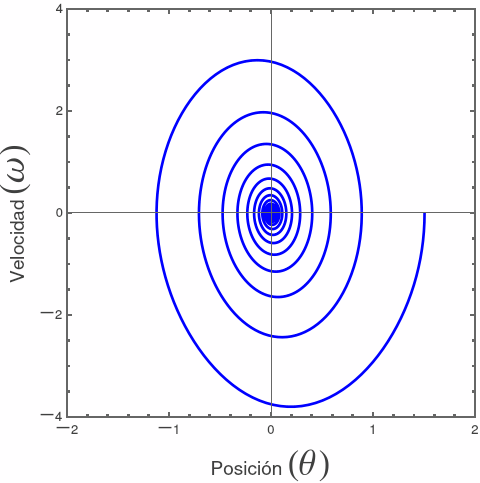
\includegraphics[width=\textwidth]{img/punto_fijo.png}
		\caption{Punto fijo: Relación entre posición y velocidad de un péndulo con fricción y resistencia al aire.}
		\label{fig:punto_fijo}
	\end{subfigure}
	\begin{subfigure}[b]{0.40\textwidth}
		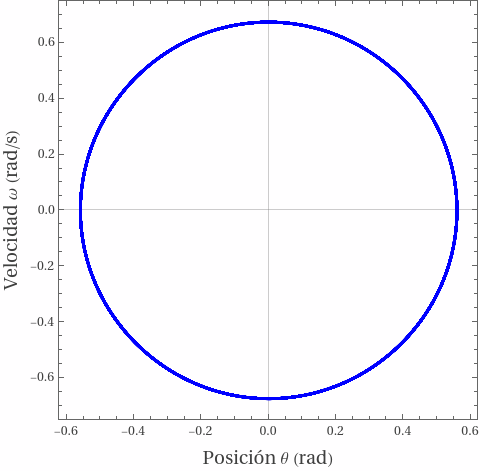
\includegraphics[width=\textwidth]{img/ciclo_limite.png}
		\caption{Ciclo límite: Movimiento oscilante de un reloj de cuarzo.}
		\label{fig:ciclo_limite}
	\end{subfigure}
	\begin{subfigure}[b]{0.40\textwidth}
		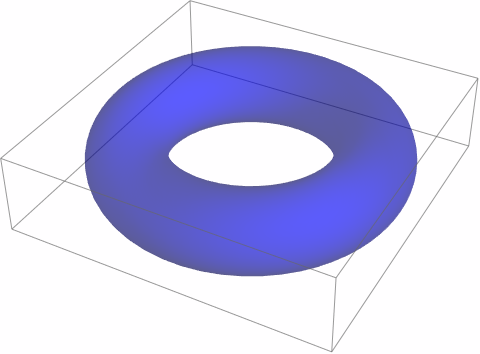
\includegraphics[width=\textwidth]{img/torus.png}
		\caption{Cuasiperiódico: Junta dos atractores de ciclo límite formando un atractor de tipo toro.}
		\label{fig:cuasi_periodico}
	\end{subfigure}
	\begin{subfigure}[b]{0.40\textwidth}
		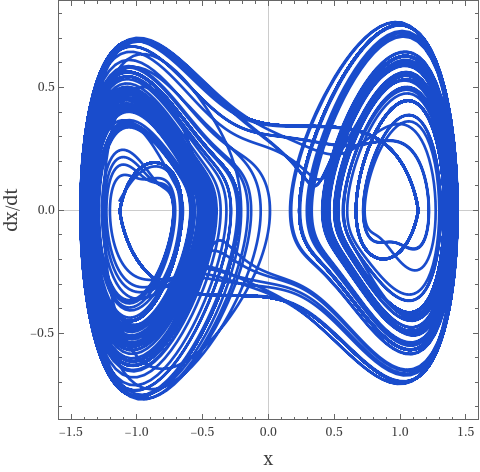
\includegraphics[width=\textwidth]{img/caotico.png}
		\caption{Extraño: Atractor de Duffing, describe el comportamiento complejo de un sistema dinámico no lineal.}
		\label{fig:caotico}
	\end{subfigure}
	\caption{Ejemplos de tipos de atractores.}
	\label{fig:atractores}
\end{figure}

\section{Sistemas complejos}

Son sistemas con muchas componentes que interactúan entre sí mediante el intercambio de materia, energía o información y que, eventualmente, sufren la acción de agentes externos \cite{complejo}. Las colonias de hormigas, el mercado bursátil, el clima, el sistema nervioso, las células y los organismos vivos son algunos ejemplos de sistemas complejos. Estos se caracterizan por tener un conjunto de elementos que interactúan entre sí con el fin de alcanzar un objetivo \cite{cs_def_1, cs_def_2}. 

Los sistemas complejos tienen dos implicaciones fundamentales: (1) Existe una influencia mutua entre sus elementos, donde el cambio afecta inevitablemente al resto de elementos, y (2) persiguen un objetivo \cite{cs_def_2}.

\begin{definition}
	
	Un sistema complejo es una entidad compuesta de partes interconectadas, de tal forma que el comportamiento colectivo es más que la suma de sus componentes individuales.
	
\end{definition}

Para entender el comportamiento de un sistema es necesario conocer los elementos y sus interacciones. Es decir, se requiere conocer los estados, valores instantáneos de todos los elementos; y sus transiciones, cambios dinámicos en los estados.

Los sistemas complejos se caracterizan principalmente por:

\begin{itemize}
	
	\item \textbf{No linealidad}: No cumple el principio de superposición, es decir, el resultado no puede expresarse como la suma de las respuestas individuales a cada estímulo por separado. Resulta difícil predecir su evolución dinámica futura \cite{cs_def_2, cs_def_3}.
	
	
	
	\item \textbf{Retroalimentación}: Las salidas pasadas influyen en las siguientes salidas. Este comportamiento hace alusión a la memoria del sistema \cite{cs_def_3}. 
	
	
	
	\item \textbf{Orden espontáneo}: Existe un orden emergente resultado de las interacciones locales no coordinadas, el cual no puede ser descrito mediante sus interacciones locales \cite{cs_def_3}.
	
	
	
	\textbf{Aparición (\textit{emergence})}: Entidades, patrones, comportamientos y propiedades emergen de la interacción de entidades más pequeñas, las cuales no exhiben estos atributos \cite{cs_def_3}.
	
	
	
	\textbf{Elementos múltiples}: Compuesto de múltiples elementos relativamente idénticos con interacciones locales \cite{cs_def_2}. 
	
\end{itemize}

\section{Modelado de sistemas complejos}

Resulta evidente que predecir el comportamiento de estos sistemas es una tarea complicada. Una aproximación es el uso de modelos científicos y matemáticos, los cuales se construyen para desarrollar procesos de inferencia sobre aspectos observados en la vida real. El modelo de inferencia se realiza para entender el sistema real observado.

El proceso, de manera simplificada, se compone de tres fases, como se observa en la figura \ref{fig:cs_cientifico}:

\begin{itemize}
	
	\item Se abstrae el sistema real a un modelo, el cual puede trascender a otros sistemas reales.
	
	
	
	\item El modelo realiza un proceso de inferencia que busca averiguar las implicaciones derivadas de las premisas.
	
	
	
	\item Los resultados se utilizan para analizar, interpretar y aplicar a un sistema real. Esta aplicación no requiere ser práctica, es una relación entre las inferencias obtenidas con el modelo y el sistema real.
	
\end{itemize}

\begin{figure}[H]
	
	\centering
	
	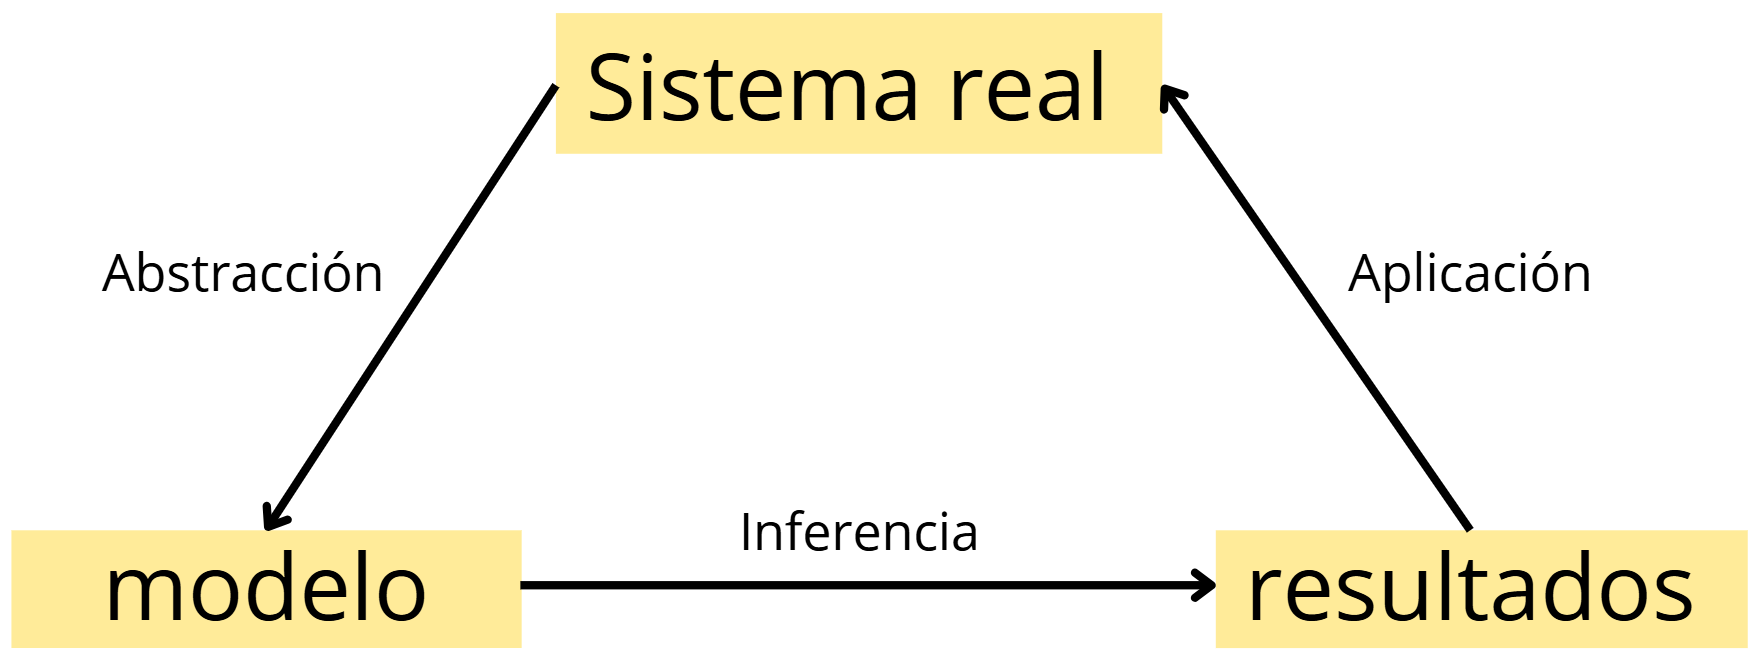
\includegraphics[width=0.6\linewidth]{img/CS_cientifico.png}
	
	\caption{Representación gráfica del modelado científico. Este proceso busca relacionar eventos del mundo real utilizando un modelo que realiza una inferencia.}
	
	\label{fig:cs_cientifico}
	
\end{figure}

Sin embargo, estos modelos suelen carecer de las herramientas necesarias que les permiten deducir las implicaciones lógicas necesarias. Es aquí donde la computación permite agilizar este proceso realizando simulaciones computacionales. 

Las computadoras permiten explorar y analizar modelos formales para resolver modelos matemáticos. Además, dado que un modelo computacional puede ser definido mediante un modelo matemático, el rol de la computación es simplificar este proceso. 

Los resultados que se obtienen al ejecutar la simulación computacional se derivan de aplicar reglas algorítmicas, por lo que se requiere expandir el proceso de abstracción y diseñar un modelo formal que será ejecutado por la computadora, como se muestra en la figura \ref{fig:cs_computacional}.

\begin{figure}[H]
	
	\centering
	
	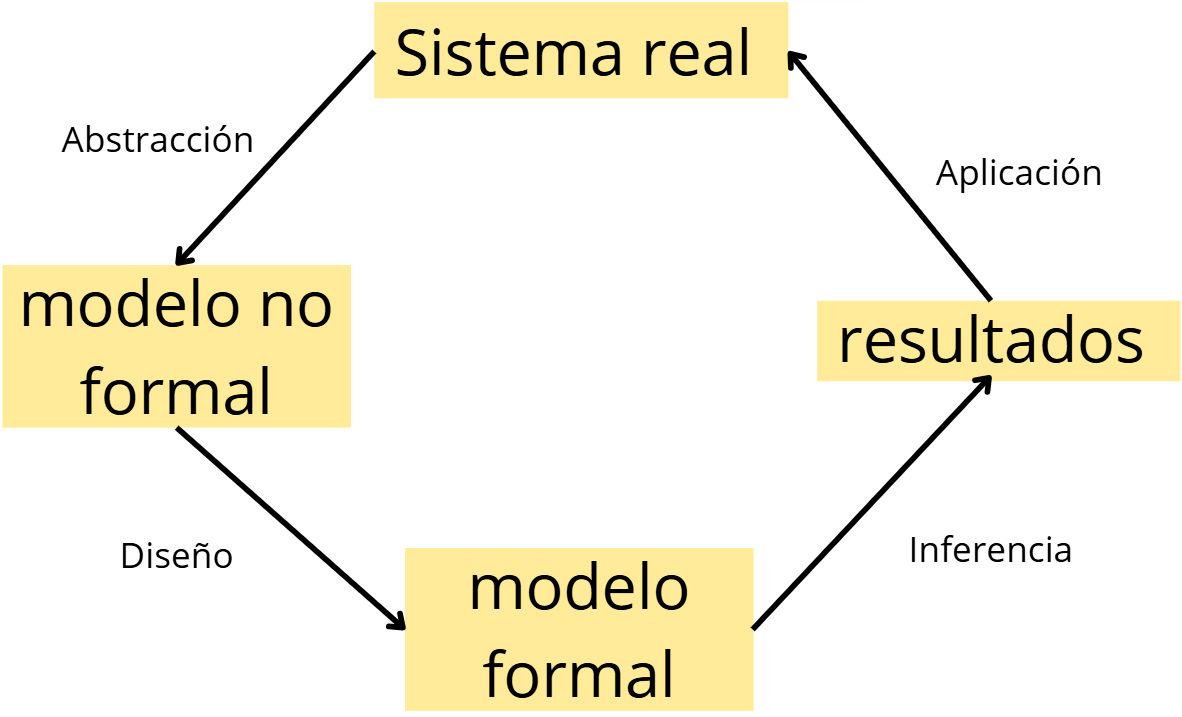
\includegraphics[width=0.6\linewidth]{img/CS_computacional.png}
	
	\caption{Representación gráfica del modelado computacional. Relaciona eventos del mundo real utilizando un modelo computacional que ayuda a agilizar el proceso de inferencia.}
	
	\label{fig:cs_computacional}
	
\end{figure}

Se requiere de un experto en el sistema real que pueda abstraer el problema y un modelador que formalice dicha abstracción para ejecutarla en una computadora que infiera los resultados, mismos que utilizará nuevamente el experto en el sistema real para entablar la relación con el sistema real \cite{modelado}.

Para modelar sistemas complejos existen múltiples herramientas; una de ellas son los autómatas celulares \cite{CS_CA}, los cuales siguen la caracterización de los sistemas complejos: elementos idénticos con interacciones locales que pueden generar orden espontáneo, comportamientos emergentes e incluso retroalimentados. 

\clearpage